%%%%%%%%%%%%%%%%%%%%%%%%%%%%%%%%%%%%%%%%%%%%%%%%%%%%%%%%%%%%%%%%%%%%%%%%%%%%%
%%%%%%%%%%%%%%%%%%%%%%%%%%%%%%%%%%%%%%%%%%%%%%%%%%%%%%%%%%%%%%%%%%%%%%%%%%%%%
\documentclass[a4paper,12pt,onecolumn]{article}

%%% Margins: 1 inch on all sides
\usepackage[a4paper,margin=2.5cm]{geometry}
%%% Packages
\usepackage{cite}
\usepackage{amsmath,amssymb,amsfonts}
\usepackage{graphicx}
\usepackage{fancyhdr}  
\usepackage{booktabs}
\usepackage{longtable}
\usepackage{array}
\usepackage{float}
\usepackage{multirow}
\usepackage{makecell}
\usepackage{ragged2e}
\usepackage{textcomp}
\usepackage{xcolor}
\usepackage{pdflscape}
\usepackage{listings}
\usepackage[most]{tcolorbox}
\newtcolorbox{highlightblock}{
	colback=yellow!20,
	colframe=yellow!20,
	boxrule=0pt,
	arc=0pt,
	left=1mm,
	right=1mm,
	top=1mm,
	bottom=1mm
}
\usepackage{etoolbox}  
\usepackage{bbm}
\usepackage{tikz}
\usetikzlibrary{positioning, arrows.meta, fit, backgrounds}
\usepackage{tcolorbox}
\usepackage{graphicx}
\usepackage{subcaption}
\usepackage{booktabs}
\usepackage{siunitx}
\tcbuselibrary{listings}
\usepackage{subcaption}
\usepackage{titling}
\bibliographystyle{IEEEtran}
\usepackage{hyperref}
\usepackage{pdfpages}
\usepackage{xcolor}
\usepackage{longtable}
\usepackage{soul}
\hypersetup{
	hidelinks,
	breaklinks=true
}

% Reduce space around figures and tables
\setlength{\textfloatsep}{10pt}   % space between floats and text
\setlength{\floatsep}{8pt}        % space between floats
\setlength{\intextsep}{8pt}       % space for in-text floats
\setlength{\parindent}{0pt}

\usepackage{xcolor}

% unchecked / not yet verified text
\sethlcolor{gray!30}

% Reduce space between caption and figure/table
\usepackage{caption}
\captionsetup{skip=4pt}

%%% Listings style
\definecolor{codegreen}{rgb}{0,0.6,0}
\definecolor{codegray}{rgb}{0.5,0.5,0.5}
\definecolor{codepurple}{rgb}{0.58,0,0.82}
\definecolor{backcolour}{rgb}{0.95,0.95,0.92}

\lstdefinestyle{mystyle}{
	backgroundcolor=\color{backcolour},
	commentstyle=\color{codegreen},
	keywordstyle=\color{magenta},
	numberstyle=\tiny\color{codegray},
	stringstyle=\color{codepurple},
	basicstyle=\ttfamily\footnotesize,
	breaklines=true,
	numbers=left,
	numbersep=5pt,
	tabsize=2
}

%%% Title spacing
\setlength{\droptitle}{-2.5cm}


%%% Title
\title{\LARGE \bf
	Technical Abstract \\
	CSI-Feedback-Driven Link Adaptation in 5G NR Downlink MIMO: A Link-Level Simulation Study}
\author{
	Kaiyuan Bao (kb784)\\
	Homerton College, University of Cambridge\\[6pt]
	\small Supervised by Prof. Albert Guillen i Fabregas and Alexander Hamilton (Nokia)
}



\begin{document}
	
	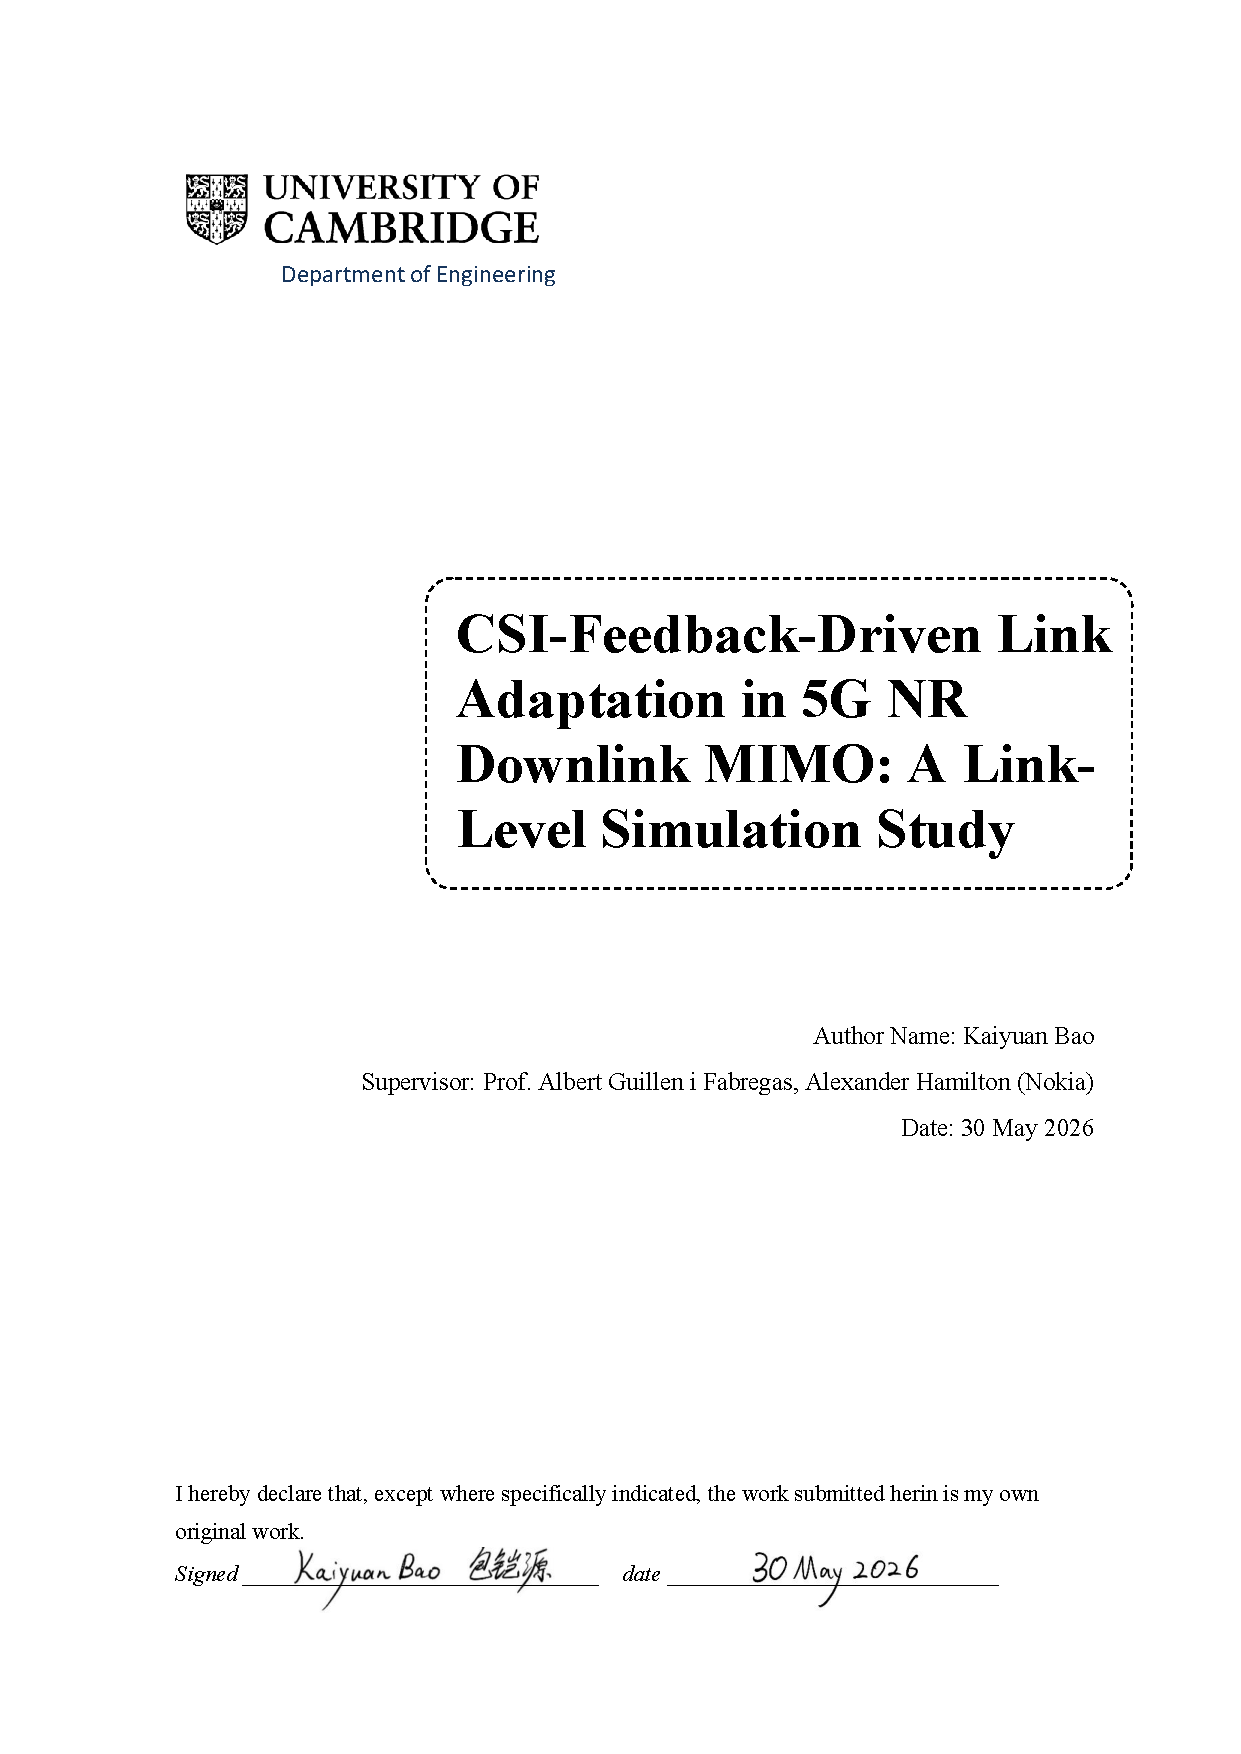
\includepdf[
	pages=1,
	pagecommand={\thispagestyle{empty}},
	fitpaper=true
	]{FrontPage.pdf}
\clearpage

\setcounter{page}{1}
\newpage
\section*{\centering Acknowledgement}
\hl{The research project is completed under the direct supervision from Prof. Albert Guillen i Fabregas from Engineering Department, University of Cambridge and Alexander Hamilton from Nokia. I sincerely thank them for their supervision, help and encouragement during the whole year, guiding me on the project.\\

The completion of the project marks the end of my four year study at Cambridge. I would like to use this opportunity to thank my parents for their huge support during my years in the UK, making it possible for me to pursue knowledge in Cambridge.}

\begin{flushright}
	Kaiyuan Bao \\ May 2026
	\end{flushright}

\newpage



	\maketitle
	\vspace{-35pt}
	\pagestyle{fancy}
	\fancyhead[L]{}   % 左侧页眉
	\fancyhead[C]{} 
	\fancyhead[R]{\rightmark}
	\renewcommand{\subsectionmark}[1]{\markright{#1}}  % 只显示标题，不显示编号
	
\thispagestyle{empty}
\section*{Background and Motivation}

\section*{Methodology}

\newpage

\thispagestyle{empty}
\section*{Key Results and Interpretation}

\section*{Conclusion}
	
\newpage
\tableofcontents
\thispagestyle{empty}
\newpage

\section*{List of Abbreviations}
\thispagestyle{empty}
\addcontentsline{toc}{section}{List of Abbreviations}

\begin{longtable}{p{3cm}p{10cm}}
	\textbf{Abbreviation} & \textbf{Definition} \\
	\hline
	
	5G      & Fifth Generation \\
	
	BLER    & Block Error Rate \\
	
	CDL     & Clustered Delay Line \\
	CP      & Cyclic Prefix \\
	CQI     & Channel Quality Indicator \\
	CSI     & Channel State Information \\
	CSI-RS  & CSI Reference Signal \\
	
	DL      & Downlink \\
	DM-RS   & Demodulation Reference Signal \\
	
	FR & Frequency Range \\
	
	gNB     & Next Generation Node B \\
	
	HARQ    & Hybrid Automatic Repeat Request \\
	
	LDPC    & Low-Density Parity-Check \\
	LOS     & Line-of-Sight \\
	
	MCS     & Modulation and Coding Scheme \\
	MIMO    & Multiple-Input Multiple-Output \\
	
	NLOS    & Non-Line-of-Sight \\
	NR      & New Radio \\
	
	OFDM    & Orthogonal Frequency Division Multiplexing \\
	
	PDCCH   & Physical Downlink Control Channel \\
	PDSCH   & Physical Downlink Shared Channel \\
	PMI     & Precoding Matrix Indicator \\

	
	QAM     & Quadrature Amplitude Modulation \\
	QPSK    & Quadrature Phase Shift Keying \\
	
	RB      & Resource Block \\
	RE      & Resource Element \\
	RI      & Rank Indicator \\
	
	SCS     & Subcarrier Spacing \\
	SINR    & Signal-to-Interference-and-Noise Ratio \\
	SISO    & Single-Input Single-Output \\
	SNR     & Signal-to-Noise Ratio \\
	

	TDL     & Tapped Delay Line \\
	
	UE      & User Equipment \\
	UL      & Uplink \\
	
\end{longtable}
\newpage

\section{Introduction}

1. 5G NR, Physical Layer, MIMO background. Why 5G needs mimo and adaptive transmission \\
2. Importance of CSI\\
3. Why fixed-rank, fixed-modulation BER curve is not enough
3. Matlab 5G toolbox simulation\\
4. Baseline scenario \\
5. RQs\\
6. Structure of my research\\

\begin{highlightblock}
	
	Mobile telecommunications have experienced rapid development over the past two decades. Starting from the deployment of third-generation (3G) systems in the early 2000s, followed by the introduction of fourth-generation long-term evolution (4G LTE) in the early 2010s, each generation has delivered substantial improvements in data rate and user experience. For end users, the most noticeable change has been the transition from limited and slow web browsing to smooth video streaming and real-time online services. These improvements were enabled by key physical-layer innovations, including the use of orthogonal frequency division multiple access (OFDMA) in 4G LTE, replacing the code division multiple access (CDMA) used in earlier systems, as well as the introduction of more advanced multi-antenna techniques \cite{Manikas}.
	
	Building upon the capabilities of 4G, the fifth-generation mobile communication system (5G) has been designed to further increase data rates, reduce latency, and support a wide range of services. Three main usage scenarios are defined for 5G: enhanced mobile broadband (eMBB), massive machine-type communications (mMTC), and ultra-reliable and low-latency communications (URLLC) \cite{EricssonBook}. Together, these scenarios impose diverse requirements on 5G, ranging from extremely high data rates to massive device connectivity, as well as stringent latency and reliability constraints. To meet these requirements, multiple-input multiple-output (MIMO) techniques play a central role. In particular, massive MIMO systems enable significant throughput gains through spatial multiplexing, null forming and beamforming \cite{Ericsson_MIMO}.
	
	The realization of these requirements relies on globally agreed technical specifications, which are defined by the Third Generation Partnership Project (3GPP), a global standardisation body established in 1998 for the development of specifications for 3G. Its scope has expanded from third-generation of cellular networks to the standardisation and continuous evolution of 4G, 5G, and technologies beyond. The first release of 5G NR, Release~15, was published by 3GPP in 2019, marking the point at which 5G NR became ready for practical implementation. In the release, core technical specifications for 5G NR were defined. 3GPP is currently continuing its work on 5G-Advanced and early studies towards 6G \cite{3GPP}. 
\end{highlightblock}
\begin{highlightblock}
	This research project aims to provide insights that can support future 3GPP standardisation discussions related to MIMO techniques in 5G and beyond. Simulations are conducted in MATLAB using a framework aligned with 3GPP specifications. This alignment includes the use of standardized channel models as well as baseline system parameters commonly adopted in 3GPP testings, such as carrier frequency and bandwidth. This report introduces the relevant background concepts, presents the adopted simulation methodology, and summarises the current progress and preliminary findings of the project.
\end{highlightblock}

\section{Background and Methodology}
\subsection{5G NR Downlink Physical Layer Overview}
	1. OFDM\\
	2. PDSCH (DL)\\
	3. DM-RS\\
	4. CSI-RS\\
	5. Slot, RB\\
	6. Definition of BER/BLER/Throughput\\
	7. Why throughput not BER
	\newpage
	
	
\subsection{MIMO Transmission and CSI Feedback}
	Specifics of CSI: PMI,RI, CQI \\
	Feedback loops\\
	How the modulation scheme/TCR/rank changes based on the feedback
	\begin{figure}[H]
		\centering
		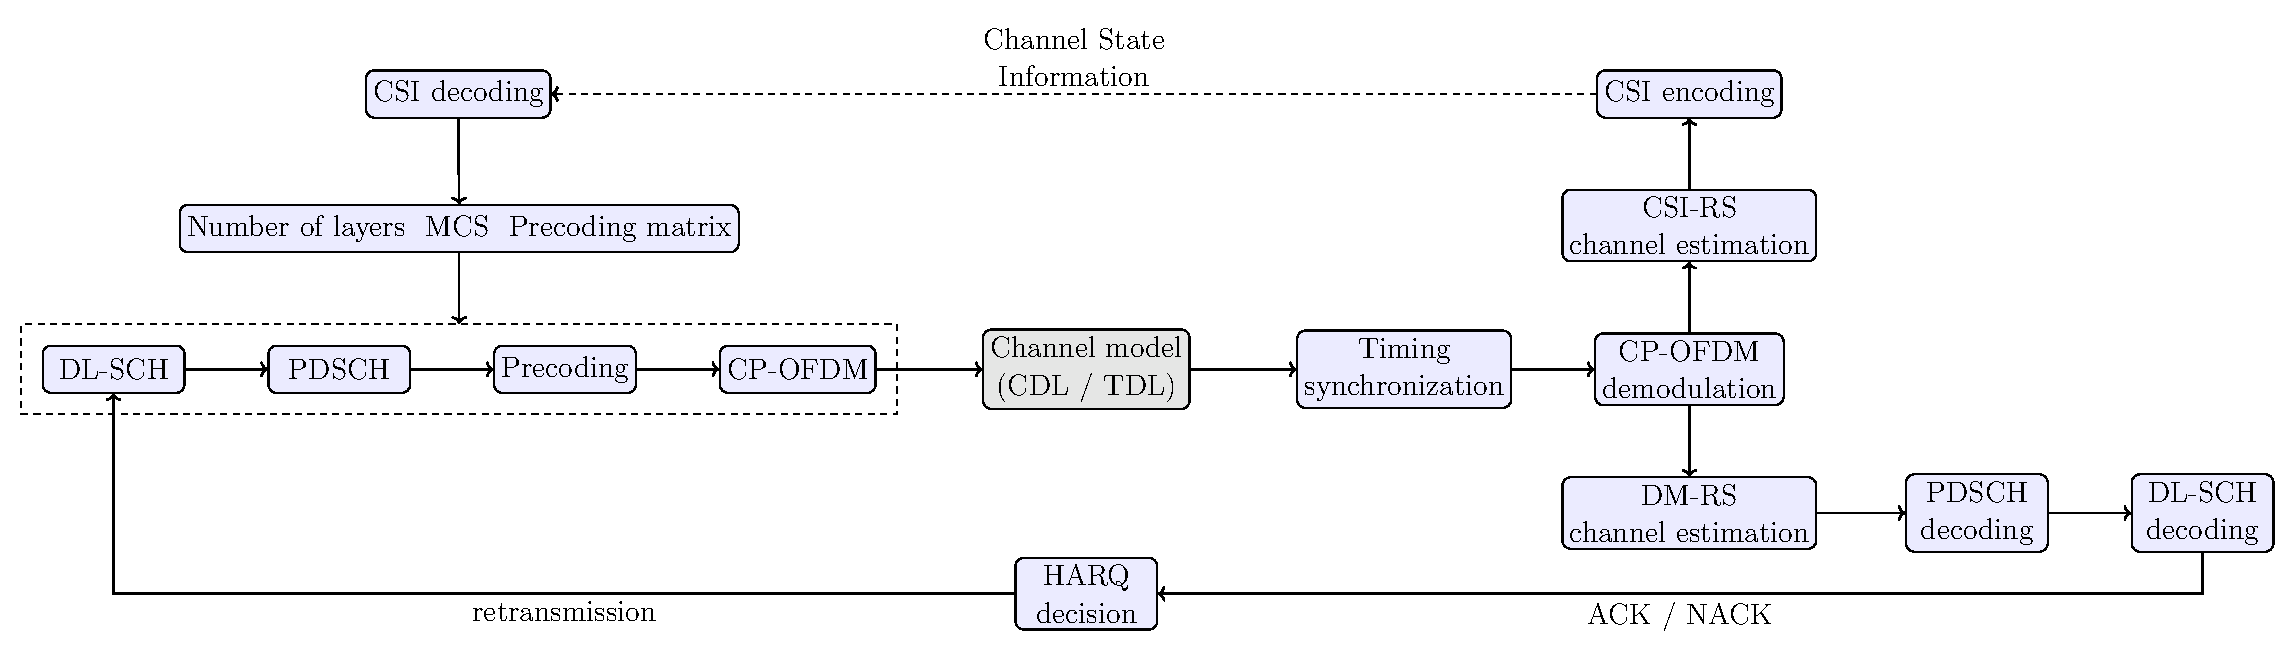
\includegraphics[width=1\linewidth]{figures/TIKZ_graph_1.pdf}
		\caption{Overview of the CSI-based downlink transmission and feedback framework, adapted from~\cite{Matlab_PDSCH_CSI}}
		\label{fig:csi_overview}
	\end{figure}
	
	\begin{highlightblock}
		As illustrated in Figure~\ref{fig:csi_overview}, the downlink transmission relies on channel state information (CSI) obtained through reference signal measurements at the receiver. The user equipment (UE) estimates the downlink channel based on CSI reference signals (CSI-RS). Based on the estimated channel, the CSI is encoded into three main feedback components: the Channel Quality Indicator (CQI), Precoding Matrix Indicator (PMI), and Rank Indicator (RI).
		
		CQI is a 4-bit indicator with values ranging from 0 to 15, representing the reported downlink channel quality. It provides an indication of the highest modulation scheme and coding rate that can be supported under a predefined target block error rate (BLER). The precoding matrix indicator (PMI) specifies the precoding matrix applied at the transmitter, while the rank indicator (RI) indicates the recommended number of transmission layers \cite{Matlab_PDSCH_CSI}.
		
		There are various parameters that affect the quality of the CSI. These include the CSI reporting periodicity, which controls how frequently the feedback is updated, as well as the reporting mode, which can be configured as wideband or subband. In addition, parameters such as the codebook type and mode, and the subband size further impact the granularity of the reported CSI. In time-varying channels, infrequent or coarse CSI reporting may lead to outdated channel knowledge at the transmitter, therefore degrading the performance of the transmission.
	\end{highlightblock}
	\begin{highlightblock}	
		The reported CSI is fed back to the transmitter and used to configure key downlink transmission parameters, including the modulation scheme, target code rate, number of transmission layers, and the precoding matrix. Using these updated parameters, the transmitter processes the data through the DL-SCH and maps it to the PDSCH, followed by precoding and CP-OFDM modulation before transmission over the wireless channel. At the receiver, the received signal is synchronised, demodulated, and decoded using demodulation reference signals (DM-RS) for coherent detection.
		
		
		There are two widely used channel models in 5G NR link-level evaluations, namely the tapped delay line (TDL) model and the clustered delay line (CDL) model. Each model has several variants designed to represent different propagation environments such as urban, suburban, and rural scenarios. The TDL model provides a simplified representation of the multipath channel and is commonly used for baseline evaluations or scenarios where spatial characteristics and multi-antenna effects are not modelled.
		
		In the TDL model, the channel is represented as a superposition of multiple discrete propagation paths (taps), each characterised by a specific delay $\tau_l$ and a path gain $h_l(t)$:
		\begin{equation}
			h(t, \tau)=\sum_{l=0}^{L-1}h_l(t)\delta(\tau-\tau_l).
		\end{equation}
		The TDL model does not represent angular or spatial features of the propagation channel. In contrast, the clustered delay line (CDL) model incorporates spatial information and therefore provides a more realistic channel description. Similar to the TDL model, the CDL model defines a set of multipath clusters characterised by relative delays and average powers. In addition, each cluster is associated with angular parameters, including the azimuth and zenith angles of departure and arrival (AoD, AoA, ZoD, and ZoA). Each cluster is further decomposed into multiple sub-rays with random initial phases and Doppler components. By modelling these spatial characteristics, the CDL channel model enables a more accurate representation of the spatial characteristics of MIMO channels, at the cost of increased complexity and higher computational cost \cite{ETSI_TDL_CDL}.
		
		In addition to CSI, 5G NR also employs hybrid automatic repeat request (HARQ) to improve the robustness of the transmission through re-transmissions. After DL-SCH decoding at the receiver, an acknowledge/negative acknowledge (ACK/NACK) signal is fed back to the transmitter, which indicates whether a re-transmission is required. In the case of a decoding failure, the transport block is re-transmitted using a different redundancy version (RV) and combined at the receiver, thus increasing the probability of successful decoding \cite{EricssonBook} \cite{MathWorks2026}.
	\end{highlightblock}

\subsection{CDL Channel Model and Doppler Shift}
	CDL model definition\\
	CDL ABCDE difference, why CDL-C default\\
	Doppler shift definition and impact
	\newpage
	
	
	
\subsection{MATLAB Simulation Framework}
	\begin{highlightblock}
		Table~\ref{tab:system_config} below summarises the baseline system and channel configuration adopted in this study, which is aligned with the assumptions commonly used in 3GPP evaluation studies, including TR~38.753~\cite{3GPPSimulationSpec}. There different mobility scenarios are considered. The low-mobility case assumes a maximum Doppler shift of 10~Hz, corresponding to a UE speed of 3 km/h, a default setting for 3GPP testing. For medium- and high-mobility cases, the 100~Hz and 390~Hz Doppler shift corresponds to the speed of approximately 30~km/h and 120~km/h respectively for a 3.5 GHz carrier frequency.
	\end{highlightblock}

		
		\begin{table}[H]
			\centering
			\caption{System and channel configuration used in the simulations}
			\label{tab:system_config}
			\begin{tabular}{ll}
				\hline
				\textbf{Parameter} & \textbf{Value} \\
				\toprule
				Carrier frequency      & FR1, 3.5 GHz \\
				Subcarrier spacing          & 30 kHz \\
				Channel bandwidth           & 106 RBs \\
				Antenna configuration       & 4 Tx, 4 Rx \\
				Maximum number of layers    & 4 \\
				Channel model               & CDL-C \\
				Mobility scenarios          & \makecell[l]{10~Hz (Default), 100~Hz, 390~Hz}\\
				Simulation type             & Downlink link-level \\
				\hline
			\end{tabular}
		\end{table}
		
		
		\begin{highlightblock}
			The CDL-C channel model is selected as it represents a typical non-line-of-sight (NLOS) urban macro environment and is widely used in 3GPP evaluation studies, while modelling spatial characteristics are essential for the study of CSI feedback. A 4$\times$4 MIMO configuration with up to four transmission layers is considered, reflecting a representative frequency range 1 (FR1) deployment while maintaining a manageable simulation complexity. This configuration allows multi-layer transmission as well as rank adaptation to be studied within a single-codeword framework, avoiding additional variability introduced by using an additional codeword, and thus enabling a clearer assessment of the effect of the CSI feedback parameters.
			
		\end{highlightblock}
		
		\begin{highlightblock}
			The full set of parameters used are shown in the Appendix section. Fig. \ref{fig:24ResouceGrid} shows the downlink resource grid of the system under such configuration. The empty....
		\end{highlightblock}
		\begin{figure}[H]
			\centering
			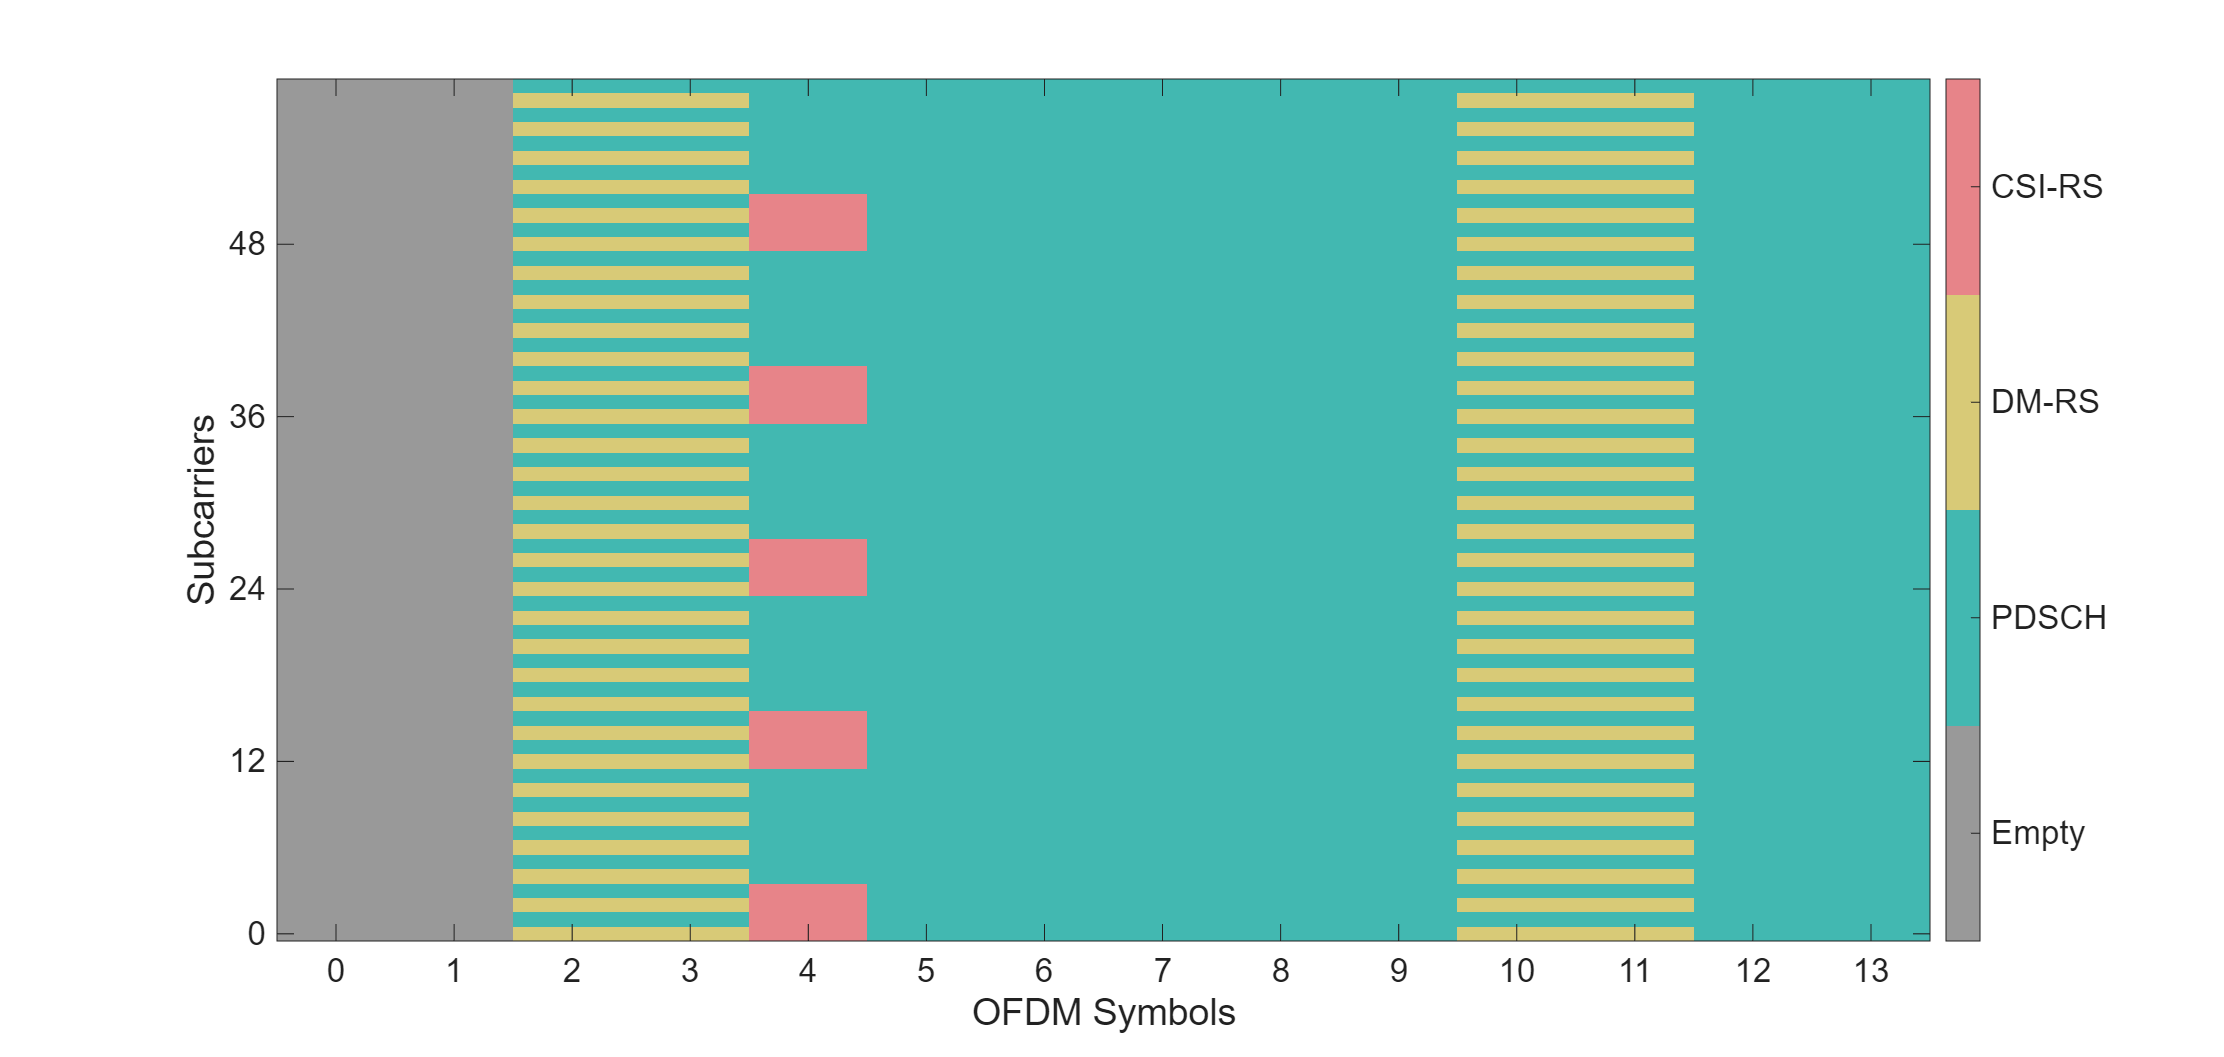
\includegraphics[width=\linewidth]{figures/24ResouceGrid.png}
			\caption{Downlink resource grid showing the allocation of PDSCH, DM-RS and CSI-RS}
			\label{fig:24ResouceGrid}
		\end{figure}
	\subsection{System Configuration and Experimental Design}
		\begin{highlightblock}
			This study focuses on investigating the impact of CSI feedback parameters on downlink transmission performance. The baseline CSI configuration follows the settings specified in relevant 3GPP specifications, including TS~38.101-4~\cite{3gpp_ts_38101_4}. Both the baseline configuration and the investigated parameter ranges are summarised in Table~\ref{tab:csi_config}. The investigated ranges represent the set of valid discrete configurations specified by 3GPP. Unless otherwise stated, all simulations use the baseline CSI configuration listed in Table~\ref{tab:csi_config}. 
		\end{highlightblock}

		\begin{table}[H]
			\centering
			\caption{Baseline CSI feedback configuration used in the simulation framework}
			\label{tab:csi_config}
			\begin{tabular}{ll}
				\hline
				\textbf{Parameter} & \textbf{Baseline setting}  \\
				\toprule
				CSI report periodicity      & 10 slots \\
				CQI reporting mode          & Wideband  \\
				PMI reporting mode          & Wideband  \\
				Subband size                & 16 RBs   \\
				RI configuration            & Adaptive \\
				Codebook type               & Type I    \\
				Codebook mode               & Mode 1   \\
				\hline
			\end{tabular}
		\end{table}
		
		
	\begin{highlightblock}
		In section \ref{sec:3}, the behaviour of the system under baseline condition will be simulated and investigated. In section \ref{sec:4}, the performance of the system under different MIMO, CDL channel configurations will be investigated, which examines whether the baseline behaviour observed in the baseline scenario remains interpretable under these changes. In section \ref{sec:5}, the CSI reporting period will be varied to analyze suitable reporting period for different scenarios and the underlying reasons behind the observations. 
		
		Only a subset of the parameters under investigation is varied in each experiment, while the remaining parameters are kept fixed at their baseline values to ensure a controlled comparison. Table \ref{tab:sim_studies} shows a brief summary of the simulation study groups that are going to be simulated. <Note that sometimes may change multiple parameters at the same time..>
	\end{highlightblock}
	
	\begin{table}[H]
		\centering
		\caption{Summary of simulation study groups and objectives}
		\label{tab:sim_studies}
		\begin{tabular}{llc}
			\hline
			\textbf{Study Group} & \textbf{Purpose} &Varied parameter \\
			\toprule
			Baseline             & CDL-C $4\times4$ reference  performance       & -- \\
			Fixed-rank controls  & Layer adaption         & RI =1, RI$\leq 2$, RI $\leq 4$\\ 
			MIMO configuration sweep        & Antenna configuration sensitivity            &  \(2 \times 2\), \(4 \times 4\), \(8 \times 4\)  \\  
			CDL profile sweep            & Channel-model robustness         & CDL-B, CDL-C, CDL-D  \\ 
			Doppler sweep        & Mobility sensitivity          & 10 Hz, 100 Hz, 390 Hz  \\
			CSI period sweep     & CSI feedback freshness              & 4, 10, 64, 160 slots \\  
			\hline
		\end{tabular}
	\end{table}
	
	\begin{table}[H]
		\centering
		\caption{Simulation execution settings}
		\label{tab:simulation_execution}
		\begin{tabular}{ll}
			\toprule
			Parameter & Value \\
			\midrule
			SNR range & $-5$ to $35$~dB, with 1~dB spacing \\
			Number of simulated frames & 1500 10-ms frames per SNR point \\
			Channel estimation & Practical channel estimation \\
			\bottomrule
		\end{tabular}
	\end{table}
\section{Baseline CSI-Feedback Downlink Behaviour}
	\label{sec:3}
	\begin{highlightblock}
		The behaviour of the system under the baseline case is tested in this section. The performance of the system as well as the role of CSI is investigated and analyzed in detail to provide a good understanding of the feedback decisions. At the second half of the section, a fixed-rank control is implemented to isolate the rank adaptation mechanism and .. the multi-layer transmission.
	\end{highlightblock}
	
	
	\subsection{Baseline CDL-C $4\times4$ Throughput Behaviour}
	\begin{highlightblock}
		Fig. \ref{fig:31StandardRun} presents the baseline downlink throughput for the CDL-C $4\times4$ MIMO configuration with adaptive CSI feedback. At the simulated range of -5~dB to 25dB, the throughput curve is increasing. The curve shows a gradual increase at low SNR, followed by a steeper transition region between approximately 5 dB and 17 dB. At 10dB, the throughput is approximately xxx Mbps. The throughput saturates at high SNR of approximately xxx Mbps. The bahaviour of the system is explained in the next subsection according to the CSI-related behaviours. This baseline provides the reference case against other scenarios compared in the subsequent simulations.
	\end{highlightblock}
		\begin{figure}[H]
			\centering
			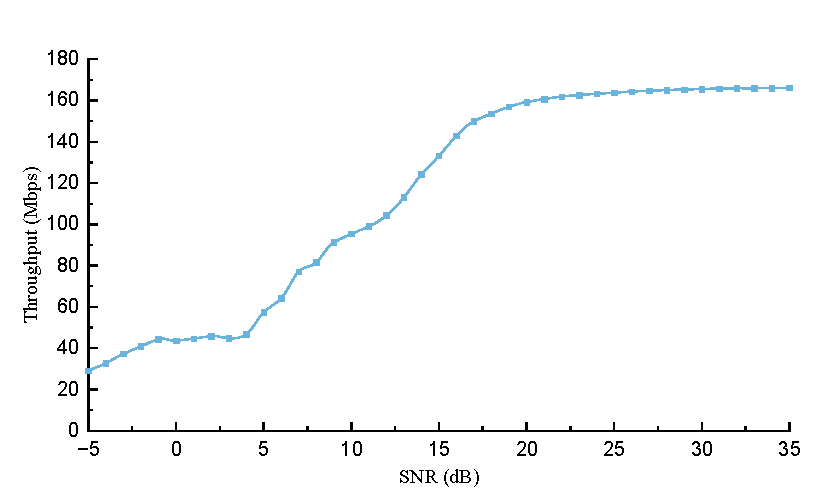
\includegraphics[width=0.75\linewidth]{figures/31StandardRun.pdf}
			\caption{Baseline downlink throughput performance for the CDL-C $4\times4$ configuration with adaptive CSI feedback}
			\label{fig:31StandardRun}
	\end{figure}
	
	\subsection{CSI-driven Link Adaptation Statistics}
	
	\begin{highlightblock}
	
		In addition to the performance of the system, the behaviour of the CSI during the transmission is shown in Fig. \ref{fig:32New_wMean} below. The four respective figures demonstrates the changes of CQI, target code rate (TCR), RI as the SNR changes as well as the use of modulation schemes at different SNR levels. CQI, TCR and RI are not fixed for each SNR testing point, but instead varies base on the real-time feedbacks and channel condition, even within subband (?). vertical bars which functions as the distribution spread indicator has been introduced to the three subfigures to characterize the consistency and variability. The bars indicate the 5th to 95th percentile range of each value range rather than the full minimum--maximum range. This choice is used to represent the typical spread of the selected CQI values while reducing the influence of rare extreme channel deep-fades or favorable fading realizations, making the results more representative.
		
		For CQI plot, as the SNR increases, the selected CQi rises gradually from 5 at low SNR to around 11 at high SNR, indicating that the link adaptation gets gradually more aggressive during the transmission due to the improved channel conditions. The peak CQI the system has every selected is 14. 
		
		Correspondingly, the target code rate of the system follows a similar trend, overall increasing from ... to nearly .... The TCR curve is not strictly increasing but instead having a oscillatory behaviour. The local minimum occur at SNR points where major change in modulation scheme occurs as the system would select a higher modulation scheme but in the meantime using a lower TCR. The two major local minimum occurs at around -3~dB and 4~dB, which corresponds to the SNR when the system switches the main modulation from QPSK to 16QAM, and from 16QAM to 64QAM respectively.
			\end{highlightblock}
			
			
		\begin{highlightblock}	

		The selected RI also changes with SNR, reflecting that the system changes the number of layers used for transmission under different channel conditions. At SNR lower than 2 dB, the system mainly selected RI = 1, representing a robust single-layer transmission. The RI increases to 2 at higher SNR, enabling steeper increase in throughput. Since the MIMO configuration is $4 \times 4$, a maximum of 4-layer transmission can be supported. However, the RI does not increase beyond 2 under this scenario, likely due to ...., partly causing the throughput to saturate to a throughput level below theoretical limit at very high SNR.
		
		For table 1 and 3 (...), three modulation schemes are supported, which are QPSK, 16QAM and 64QAM. 256 QAM is only supported when (...) and is uncommonly used due to its high requirement on channel condition. At very low SNR, the main modulation scheme is QPSK. As the SNR increases, QPSK quickly disappears and 16 QAM becomes dominant. For SNR higher than 10dB, 64QAM modulation dominates. The change in modulation scheme is gradual instead of abrupt, where the higher order modulation scheme will gradually be used more frequently as the SNR increases. The system uses 64 QAM for around 90\% of the cases, while the rest of the time using 16 QAM, likely during unusual channel degradation such as deep fade.
			\end{highlightblock}



	\begin{figure}[H]
		\centering
		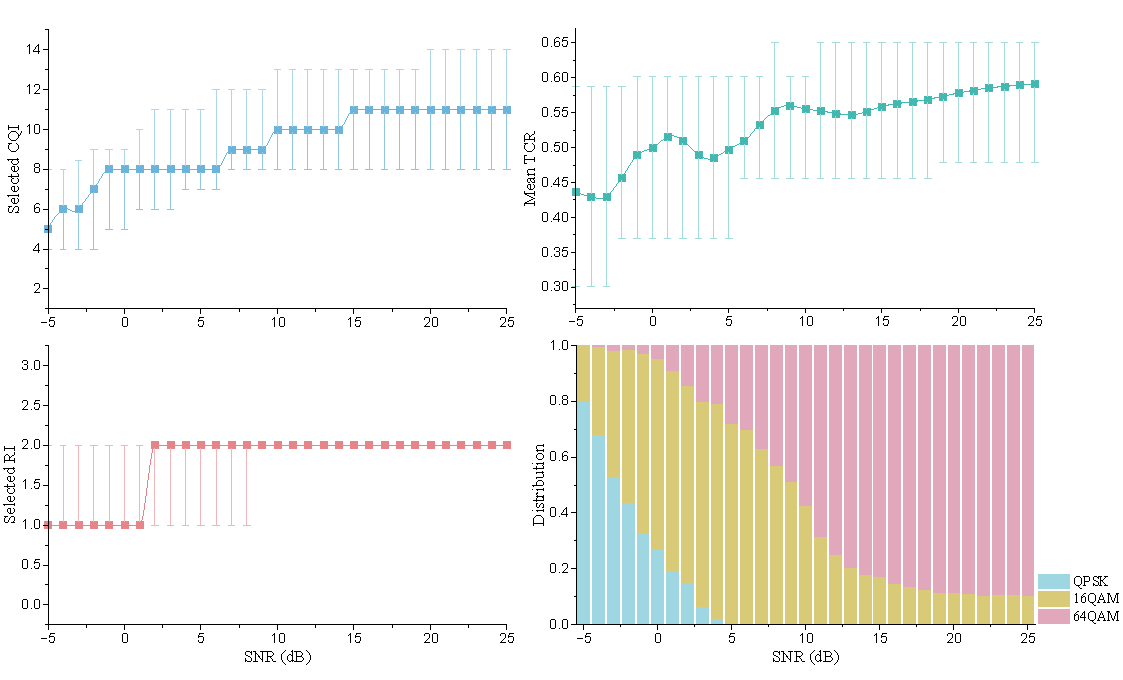
\includegraphics[width=1\linewidth]{figures/32New_wMean.pdf}
		\caption{CSI-driven link adaptation behaviour across SNR}
		\label{fig:32New_wMean}
	\end{figure}
	
		\begin{highlightblock}
			Explain why shape of throughput curve ....
		\end{highlightblock}
	\newpage
	\subsection{Fixed-Rank Controls}

	
	\begin{highlightblock}
		Figure~\ref{fig:33Layer124} compares the downlink throughput under different rank-restriction configurations. The RI $\leq 4$ case corresponds to the original baseline, where up to four transmission layers are permitted. The RI $\leq 2$ case restricts the adaptive RI selection to at most two layers, while the RI $=1$ case forces single-layer transmission.
		
		The RI $\leq 4$ and RI $\leq 2$ curves are almost identical across the full SNR range. This confirms that, under the configuration considered here, allowing more than two layers provides little additional throughput benefit. This observation is consistent with the link adaptation statistics in Figure~\ref{fig:32New_wMean}, where the selected RI increases from one to two at low-to-moderate SNR but does not increase beyond RI = 2. 
		
		The fixed RI $=1$ curve behaves differently. At low SNR, single-layer transmission can be slightly more robust than two-layer transmission, leading to lower BER and therefore higher throughput. However, as SNR increases, the lack of spatial multiplexing becomes the dominant limitation. The RI $=1$ throughput saturates at around xxx Mbps starting from around 17~dB, whereas the adaptive RI cases reach approximately xxx Mbps. This shows that adaptive multi-layer transmission is essential for achieving the high-SNR throughput gain. The higher-rank transmission beyond two layers is not effectively exploited in this baseline scenario, but the usage of adaptive layer transmission will be even bigger in a richer <?> channel that supports more independent paths <?>.
		
			\begin{figure}[H]
			\centering
			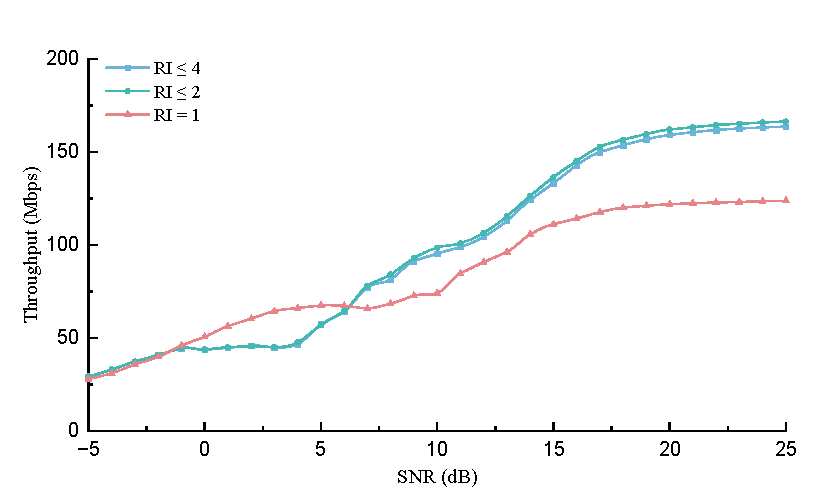
\includegraphics[width=0.75\linewidth]{figures/33Layer124.pdf}
			\caption{Downlink throughout performance under different maximum layer configurations}
			\label{fig:33Layer124}
		\end{figure}
	\end{highlightblock}
	
	\newpage
	\subsection{Summary of Baseline Findings}
	1. The above result is the baseline
	2. Examines the impact of CSI and how it actually works
	
	\newpage
	
	
	\section{Robustness across MIMO and Channel Configurations}
	\label{sec:4}
		\begin{highlightblock}
			This chapter examines if the baseline behaviour observed in the previous section remains consistent under different MIMO and CDL channel configurations. The aim of this part is to check whether the main link-adaptation trends remain interpretable when the spatial and channel conditions are changed. 
		\end{highlightblock}

		\subsection{Antenna Configuration Sweep}
		
		\begin{highlightblock}
		 Figure~\ref{fig:51AntennaNew} compares the downlink throughput performance under different MIMO antenna configurations. The $4\times4$ case corresponds to the baseline configuration discussed in the previous chapter. Two additional configurations $2 \times 2$ and $8\times4$ are tested.
		 
		 Despite the fact that, as also shown in the previous section that the maximum number of layers that are actually been used are 2, having a larger antenna array leads to better performance of the system due to ..... 
		 
		 The $2\times2$ configuration leads to a noticeably lower throughput across the SNR ranges as compared to the baseline $4\times4$ configuration and saturates at around 90 Mbps. This is as expected, as a smaller antenna configuration leads to  fewer spatial degrees of freedom.
		 
		 Oppositely, the $8\times4$ case can in general lead to better performance of the system. At low-to-medium SNR region, the increase in Tx antennas leads to higher throughput than the baseline,  suggesting that the larger transmit array improves the effective channel quality and allows the link adaptation algorithm to select more efficient transmission parameters at lower SNR values <?>. The throughput for baseline outperforms $8\times4$, however, when the SNR is above 17dB, reaching approximately xxx Mbps compared with around xxx Mbps for $8\times4$. 
		 
		 This difference should not be interpreted as evidence that $8\times4$ MIMO is inherently worse at high SNR. The saturated performance of the system is a result of the CSI feedback, which often lead to slightly different CQI, thus different TCR, layer or even transmission schemes. The result here indicates that the additional transmit antennas are not fully converted into a higher peak throughput under the current CSI feedback configuration. In this setup, the benefit of $8\times4$ is mainly observed as an SNR gain of approximately 5~dB in the low-to-medium SNR region rather than as a higher saturation throughput.
		\end{highlightblock}
		\begin{figure}[H]
			\centering
			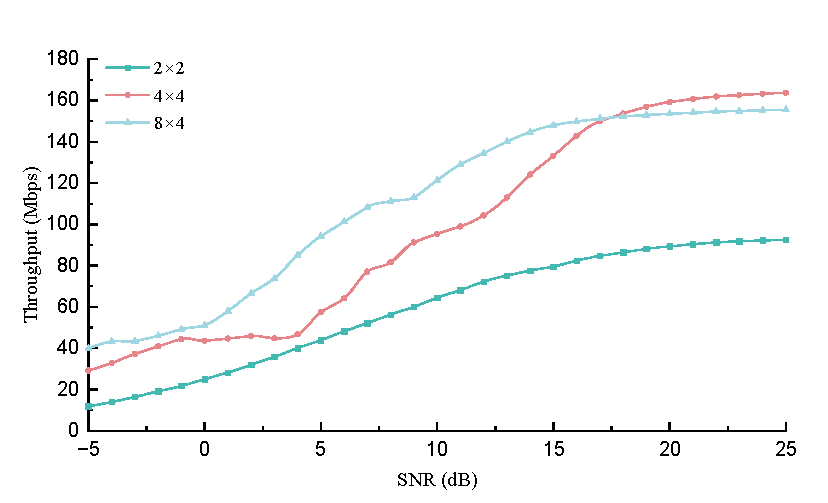
\includegraphics[width=0.75\linewidth]{figures/51AntennaNew.pdf}
			\caption{Downlink throughout performance under different MIMO configurations \hl{Still need to check 1x1 and 4x8 and 8x8? results}}
			\label{fig:51AntennaNew}
		\end{figure}
		
		\subsection{CDL Channel Profile Sweep}
		
		\begin{highlightblock}
		The second check varies the CDL channel profile while keeping the baseline $4\times4$ MIMO configuration and CSI feedback settings unchanged. 
		
		Figure~\ref{fig:52CDLBCD} compares the downlink throughput performance under CDL-B, a typical NLOS channel, and CDL-D, a typical LOS channel with the baseline. The CDL-C case corresponds to the baseline configuration. 
		
		Across all three profiles, the throughput increases with SNR and eventually approaches a profile-dependent saturation level, showing that the general link-adaptation behaviour remains interpretable. However, the transition region and high-SNR throughput differ significantly between channel profiles.
		
		The CDL-D profile achieves the best low-to-medium SNR performance and reaches the high-throughput region earlier than CDL-C. In the transition region, CDL-D shows an SNR gain of approximately 5--6~dB relative to the CDL-C baseline at comparable throughput levels. This appears as a leftward shift of the throughput curve, indicating that the same throughput can be achieved at a lower SNR. At high SNR, CDL-D and CDL-C converge to similar saturation throughput levels, with CDL-D only slightly above the baseline.
		
		In contrast, the CDL-B profile increases more gradually and saturates at a much lower throughput, around 80~Mbps. This indicates that, under the current CSI feedback and receiver configuration, the CDL-B channel does not support the same level of effective spatial multiplexing or link adaptation gain as CDL-C and CDL-D. Therefore, the high-SNR throughput ceiling is strongly affected by the channel profile, not only by the nominal antenna configuration.
		
		Overall, the CDL profile sweep shows that the qualitative shape of the throughput curve is robust, but the achievable throughput and required SNR are channel-dependent. CDL-D mainly improves the transition-region SNR requirement, CDL-C provides the baseline high-throughput behaviour, while CDL-B represents a more limiting channel condition under the current setup.
		\end{highlightblock}
		
		\begin{figure}[H]
			\centering
			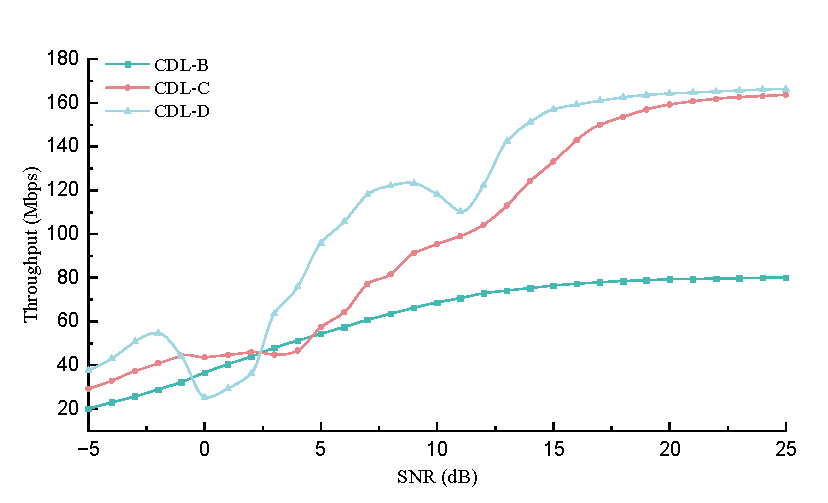
\includegraphics[width=0.75\linewidth]{figures/52CDLBCD.pdf}
			\caption{Downlink throughout performance under different CDL channel models}
			\label{fig:52CDLBCD}
		\end{figure}
		\subsection{One-layer Control Experiments}
		\begin{figure}[H]
		\centering
		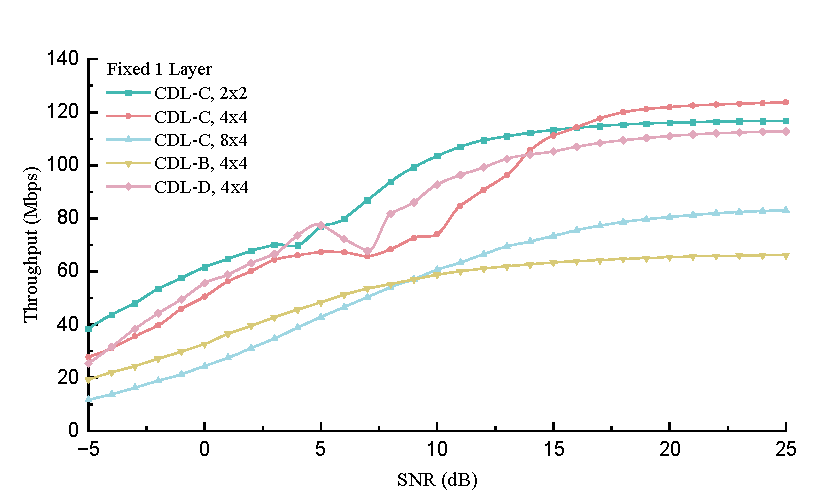
\includegraphics[width=0.75\linewidth]{figures/53Fixed1Layer.pdf}
		\caption{Downlink throughout comparison under fixed one-layer transmission \hl{Some issue with [2x2] and [8x4] curves, re-simulate}}
		\label{fig:53Fixed1Layer}
	\end{figure}
	
	
	
\section{Impact of Mobility and CSI Reporting Periodicity}
	\label{sec:5}
	\subsection{Doppler Shift under Default CSI Reporting Period}
	\begin{figure}[H]
		\centering
		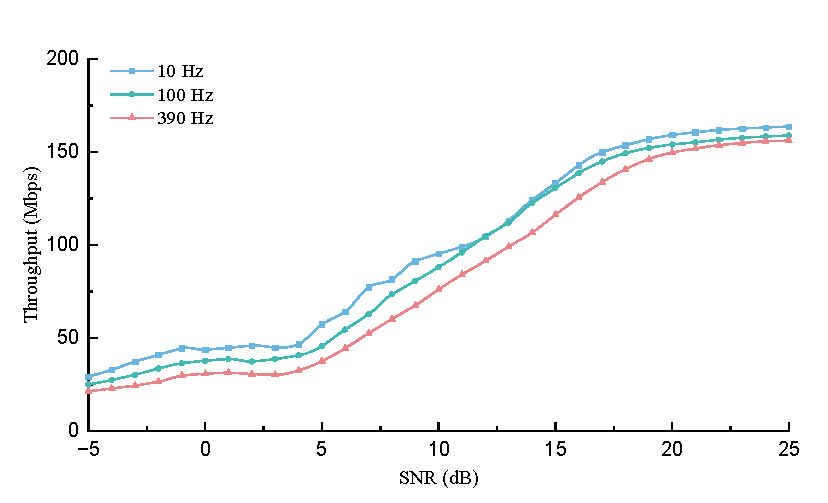
\includegraphics[width=0.75\linewidth]{figures/41Throughput_Speed.pdf}
		\caption{Impact of Doppler shift on downlink throughput}
		\label{fig:41Throughput_Speed}
	\end{figure}
	


	\begin{table}[H]
		\centering
		\caption{Interpolated SNR values at selected target throughput levels}
		\label{tab:snr_interpolation}
		
		\begin{tabular}{cccc}
			\midrule
			\textbf{\makecell{Target Throughput\\(Mbps)}} & \textbf{\makecell{SNR 10 Hz \\(dB)}} & \textbf{\makecell{SNR 100 Hz \\(dB)}} & \textbf{\makecell{SNR 390 Hz \\(dB)}} \\
			\toprule
			50  & 4.31  & 5.50  & 6.69  \\
			80  & 7.66  & 8.91  & 10.50 \\
			110 & 12.66 & 12.73 & 14.35 \\
			140 & 15.70 & 16.23 & 17.89 \\
			\bottomrule
		\end{tabular}
		
		\vspace{0.3em}
		\raggedright
		\footnotesize{$^\dagger$ SNR values obtained using linear interpolation.}
		
	\end{table}
	



	\subsection{Reporting Periodicity at Low and High mobility}
	
			\begin{figure}[H]
				\centering
				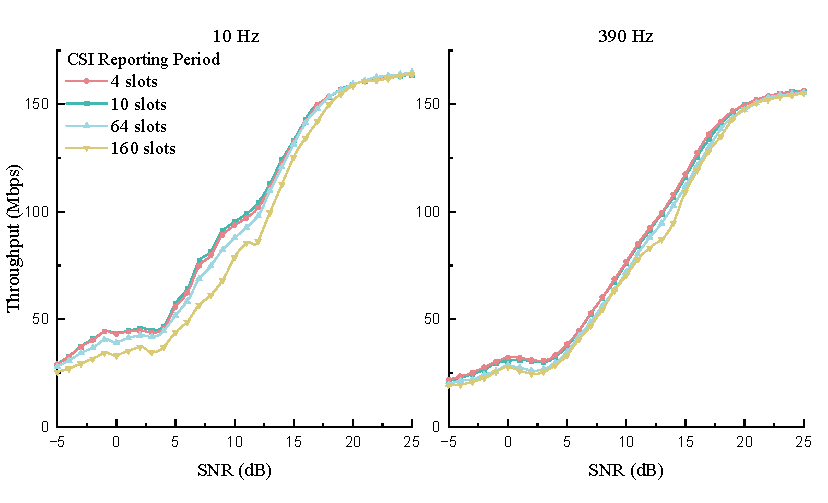
\includegraphics[width=\linewidth]{figures/42PO.pdf}
				\caption{Downlink throughput performance under different CSI reporting periods for low- and high-mobility scenarios}
				\label{fig:42PO}
			\end{figure}
			
		\begin{highlightblock}
				Reporting period of 10 slots are used as the baseline $P_0=10$. For each Doppler frequency \(f_D\), the reference peak throughput is defined as
			\begin{equation}
				R^{\max}_{f_D,P_0}
				=
				\max_{\gamma} R_{f_D,P_0}(\gamma),
			\end{equation}
			where \(R_{f_D,P}(\gamma)\) is the measured downlink throughput at SNR \(\gamma\) under CSI reporting period \(P\). The target throughput level used for comparison is 50\% of the reference peak throughput is $
				0.5 R^{\max}_{f_D,P_0}
				$. \\

			Therefore, the SNR required for each reporting period to reach the target throughput is obtained by linear interpolation as 
			$\gamma_{f_D,P}(0.5R^{\max}_{f_D,10})$. The relative SNR penalty or gain with respect to the baseline CSI report is then
			\begin{equation}
				\Delta \gamma_{f_D,P}
				=
				\gamma_{f_D,P}(0.5R^{\max}_{f_D,10})
				-
				\gamma_{f_D,10}(0.5R^{\max}_{f_D,10}).
			\end{equation}
			Positive values indicate an SNR penalty, while negative values indicate an SNR gain.
		\end{highlightblock}
		
		\begin{table}[H]
			\centering
			\caption{SNR required to reach 50\% of the baseline reference peak throughput}
			\label{tab:csi_period_snr_required}
			\begin{tabular}{llcc}
				\midrule
				\textbf{Doppler} & \textbf{CSI period} & \(\gamma_{50\%}\) & \(\Delta\gamma\) \\
				\toprule
				10 Hz  & 4 slots   & 8.2 dB & 0.1 dB \\
				10 Hz  & 10 slots  & 8.1 dB & -- \\
				10 Hz  & 64 slots  & 9.0 dB & 0.9 dB \\
				10 Hz  & 160 slots & 10.5 dB & 2.4 dB \\
				\midrule
				100 Hz & 4 slots   & 8.5 dB & -0.5 dB \\
				100 Hz & 10 slots  & 9.0 dB & -- \\
				100 Hz & 64 slots  & 11.0 dB & 2.0 dB \\
				100 Hz & 160 slots & 10.8 dB & 1.8 dB \\
				\midrule
				390 Hz & 4 slots   & 10.3 dB & -0.1 dB \\
				390 Hz & 10 slots  & 10.4 dB & -- \\
				390 Hz & 64 slots  & 10.8 dB & 0.4 dB \\
				390 Hz & 160 slots & 11.2 dB & 0.8 dB \\
				\bottomrule
			\end{tabular} \\
			$^\dagger$ Reference peak throughput values used: 
			163.9 Mbps at 10~Hz, 161.0 Mbps at 100~Hz, 158.0 Mbps at 390~Hz.
			
		\end{table}
		
		\newpage
	\subsection{Joint Interpretation: CSI Freshness}
	Summarize 4.2 and 4.3 
	CSI feedback should not be evaluated only by its granularity or reporting frequency. Its value depends on whether the reported channel state remains relevant over the time scale of channel variation.
	\subsection{Discussion of Feedback Overhead and Practical Trade-Off}
	1. What exactly is the cost of CSI  feedback
	2. Under what scenarios are frequent CSI report actually useful
	
	\newpage
	




\section{Discussion and Conclusion}
	\subsection{Interpretation of Results}
	
	\subsection{Limitations}
	
	\subsection{Future Work}
	
\newpage
\section{References} \let\refname\relax
\thispagestyle{empty}
	\vspace*{-1cm}
	\begingroup
	\bibliography{FinalReport}
\endgroup

\newpage
\section{Appendix}
\thispagestyle{empty}
\subsection{Risk Assessment}

\subsection{Ethical Statement}

\subsection{Declaration of the use of generative AI}

\newpage
\thispagestyle{empty}
\subsection{Detailed Baseline Simulation Configuration}


\begin{table}[H]
	\centering
	\caption{\hl{Baseline simulation parameters, adapted from 3GPP TR 38.753 where applicable}}
	\begin{tabular}{|ll|l|}
		\hline
		\multicolumn{2}{|l|}{Parameter}                                                                                                                                   & Value               \\ \hline
		\multicolumn{2}{|l|}{Duplex mode}                                                                                                                                 & TDD                 \\ \hline
		\multicolumn{2}{|l|}{FR / Carrier frequency}                                                                                                                      & FR1, 3.5GHz         \\ \hline
		\multicolumn{2}{|l|}{Maximum Doppler shift}                                                                                                                                    &  10~Hz                  \\ \hline
		\multicolumn{2}{|l|}{Channel Bandwidth / SCS}                                                                                                                     & 40Mhz / 30kHz       \\ \hline
		\multicolumn{2}{|l|}{Maximum allowed rank}                                                                                                                                        & 4                   \\ \hline
		\multicolumn{2}{|l|}{Antenna configuration}                                                                                                                       & 4Tx4Rx              \\ \hline
		\multicolumn{2}{|l|}{Channel model}                                                                                                                               & CDL-C               \\ \hline
		\multicolumn{2}{|l|}{Delay spread}                                                                                                                               & 300~ns               \\ \hline
		\multicolumn{2}{|l|}{\begin{tabular}[c]{@{}l@{}}Codebook configuration \\ for PDSCH and DMRS\end{tabular}}                                                        & Single Panel Type I \\ \hline
		\multicolumn{2}{|l|}{MCS table}                                                                                                                               & Table 1 (64 QAM)               \\ \hline
		\multicolumn{1}{|l|}{\multirow{4}{*}{PDSCH configuration}}      & Mapping type                                                                                    & Type A              \\ \cline{2-3} 
		\multicolumn{1}{|l|}{}                                          & k0                                                                                              & 0                   \\ \cline{2-3} 
		\multicolumn{1}{|l|}{}                                          & Starting symbol                                                                                 & 2                   \\ \cline{2-3} 
		\multicolumn{1}{|l|}{}                                          & Length                                                                                          & 12                  \\ \hline
		\multicolumn{1}{|c|}{\multirow{3}{*}{PDSCH DMRS configuration}} & DMRS Type                                                                                       & Type 1              \\ \cline{2-3} 
		\multicolumn{1}{|c|}{}                                          & Number of additional DMRS                                                                       & 1                   \\ \cline{2-3} 
		\multicolumn{1}{|c|}{}                                          & \begin{tabular}[c]{@{}l@{}}Max. number of OFDM \\ symbols for DL front loaded DMRS\end{tabular} & 2                   \\ \hline

	\end{tabular}
\end{table}

% Please add the following required packages to your document preamble:
% \usepackage{multirow}
\begin{table}[H]
	\centering
	\caption{\hl{Baseline CSI simulation parameters, adapted from 3GPP TR 38.753 where applicable}}
	\begin{tabular}{|ll|l|l|}
		\hline
		\multicolumn{2}{|l|}{Parameter}                                                                                                               & Unit & Value    \\ \hline
		\multicolumn{1}{|l|}{\multirow{3}{*}{\begin{tabular}[c]{@{}l@{}}NZP CSI-RS for \\ CSI acquisition\end{tabular}}} & CSI-RS resource type       &      & Periodic \\ \cline{2-4} 
		\multicolumn{1}{|l|}{}                                                                                           & Density                    &      & 1        \\ \cline{2-4} 
		
		\multicolumn{1}{|l|}{}                                                                                           & Symbol location                   &      & 4        \\  \cline{2-4} 
		\multicolumn{1}{|l|}{}                                                                                           & Subcarrier location                   &      & 0        \\ \cline{2-4} 
		
		\multicolumn{1}{|l|}{}                                                                                           & CSI-RS interval and offset & slot & 10, 1    \\ \hline
		\multicolumn{2}{|l|}{CQI}                                                                                                                     &      & Wideband \\ \hline
		\multicolumn{2}{|l|}{PMI}                                                                                                                     &      & Wideband \\ \hline
		\multicolumn{2}{|l|}{CQI/RI/PMI delay}                                                                                                        & ms   & 7        \\ \hline
	\end{tabular}
\end{table}

\end{document}
